% !TEX TS-program = pdflatex
% !TEX encoding = UTF-8 Unicode

% This file is a template using the "beamer" package to create slides for a talk or presentation


\documentclass[xcolor=table]{beamer}
\usepackage{setspace}
 \usepackage{tabularx} 
\usepackage{arydshln}
%\setbeamersize{text margin left=5pt,text margin right=5pt}
%\definecolor{LRed}{rgb}{1,.8,.8}
%\definecolor{MRed}{rgb}{1,.6,.6}
\definecolor{HRed}{rgb}{1,.2,.2}
\usepackage{mathtools}

\setbeamertemplate{footline}[frame number]
\mode<presentation>
{
  \usetheme{Darmstadt}
  % or ...

  \setbeamercovered{transparent}
  % or whatever (possibly just delete it)
}

\usepackage{tikz}
%\usepackage{chronosys}
\usepackage{breqn}

\usepackage{bbm}
\usepackage[english]{babel}
% or whatever
\usepackage{color,soul}
\usepackage[utf8]{inputenc}
% or whatever
\usepackage{color, colortbl}
\usepackage{times}
\usepackage[T1]{fontenc}
% Or whatever. Note that the encoding and the font should match. If T1
% does not look nice, try deleting the line with the fontenc.
\newcommand\tab[1][1cm]{\hspace*{#1}}
\usepackage{xcolor}

\newcommand{\highlight}[1]{%
  \colorbox{yellow!50}{$\displaystyle#1$}}
\title[Effects of a Minimum Wage Increase on Restaurants] % (optional, use only with long paper titles)
{\large Effects of a Minimum Wage Increase on Restaurants: \\\
 Price Pass Through and Beyond}

%\subtitle
%{Include Only If Paper Has a Subtitle}

\author[Chelsea Crain] % (optional, use only with lots of authors)
{}
% - Give the names in the same order as the appear in the paper.
% - Use the \inst{?} command only if the authors have different
%   affiliation.

\institute[] % (optional, but mostly needed)


\date % (optional, should be abbreviation of conference name)
{Chelsea Crain\\
University of Iowa\\
\today \\

}



\begin{document}



\begin{spacing}{1.2}
\begin{frame}
  \titlepage
\end{frame}



\begin{frame}{Overview}
 How do restaurant prices change in response to increases in the minimum wage?
\begin{itemize}
\item Significant price pass through consistent with literature
\item Heterogeneity across restaurant characteristics
\item Heterogeneity across item type
\end{itemize}
 How is customer perceived quality of restaurants affected by a minimum wage increase?
\begin{itemize}
\item Good restaurants get better
\item Bad restaurants get worse
\end{itemize}
 Do border effects have an impact on price pass through?
\begin{itemize}
\item Yes, in areas with a minimum wage increase
\end{itemize}
\end{frame}

\section{Background \& Policies}

\begin{frame}{Minimum Wage Background}
Minimum wage adjusted for inflation over time

\bigskip 

\centering
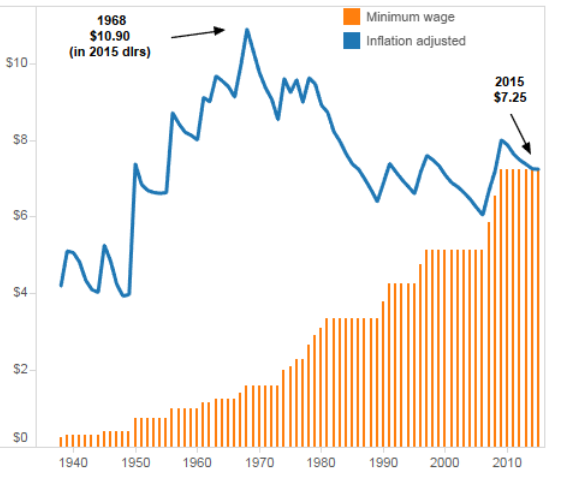
\includegraphics[width=2.8in]{cnbc_graph.png}

\raggedleft
\tiny{Published by CNBC, source: BLS}
\end{frame}

\begin{frame}{Minimum Wage Background}
Recent news
\begin{itemize}
\item ``The `Fight For 15' Continues in Maryland General Assembly'' (CBS, March `17)
\item ``'Fight For 15' organizers file lawsuit against City of Memphis'' (ThinkProgress, March `17)
\item ``New Illinois \$15 minimum wage bill reopens wage fight'' (Chicago Tribune, March `17)
\item ``The Fight for \$15 and the Rise of the Machines'' (American Thinker, March `17)
\item ``Thanks to `Fight for \$15' Minimum Wage, McDonald's Unveils Job-Replacing Self-Service Kiosks Nationwide'' (Forbes, Nov `16)
\end{itemize}
\end{frame}


\begin{frame}{Related Work on Minimum Wage}

Card and Kruger (1995), Aaronson (2001), MacDonald and Aaronson (2006), Basker and Khan (2013), Dube and Naidu (2007), Colla, Dow and  Dube (2011), Aaronson, French and MacDonald (2008), Neumark and Washer (1994), Abowd et. al (2000), Burkhauser et. al (2000), Zavodny (2000), Sbia (2006), Flinn (2006), Card and Kruger (1995), Manning (1995), Rebitzer and Taylor (1995), Burdett and Mortenson (1998), Bhaskar and To (1999), Ahn and Arcidiacono (2003)
 
\end{frame}

\begin{frame}{This Study}
\begin{itemize}
\item Six contiguous East Coast states increased minimum wage at the start of 2017
\item Variation in minimum wage across states and within states
\item Analyze full menus from two online sources
\item Analyze restaurant specific characteristics 
\begin{itemize}
\item Quality
\item Border effects
\end{itemize}

\end{itemize}
\end{frame}



\begin{frame}{Minimum Wage Laws}
\footnotesize
\centering
\begin{tabular}{ c c c c c c c} \\ \hline \hline
&  \multicolumn{3}{c}{Regular Minimum Wage} & \multicolumn{3}{c}{Tipped Minimum Wage}\\
 Area & `16  & `17  & $\% \Delta$ & `16 & `17 &  $\% \Delta$  \\ \hline \hline
 NYC \& FF & \$10.50 & \$12.00 & 14.29\%& - & - & - \\
 NY Upstate \& FF  & \$9.75 & \$10.75 & 10.26\% & - & -& - \\
 \\
 \\
 \\
 \\
 \\
 \\
 \\
 \\
 \\
%NYC \& Lg & \$9.00 & \$11.00 & 22.22\% \\
%NYC \& Sm & \$9.00 & \$10.50 & 16.67 \% \\
%NYC MSA & \$9.00 & \$10.00 & 11.11\% \\
%NY Upstate & \$9.00 & \$9.70 & 7.78\% \\
%Connecticut & \$9.60 & \$10.10 & 5.21\% \\
%New Jersey &  \$8.38 & \$8.44 & 0.72\% \\
%Massachusetts & \$10.00 & \$11.00 & 10.00\% \\
%Pennsylvania &  \$7.25 & \$7.25 & 0.00\% \\
%Vermont &  \$9.60 & \$10.00 & 4.2\% \\
\end{tabular}
\end{frame}

\begin{frame}{Minimum Wage Laws}
\footnotesize
\centering
\begin{tabular}{ c c c c c c c} \\ \hline \hline
&  \multicolumn{3}{c}{Regular Minimum Wage} & \multicolumn{3}{c}{Tipped Minimum Wage}\\
 Area & `16  & `17  & $\% \Delta$ & `16 & `17 &  $\% \Delta$  \\ \hline \hline
 NYC \& FF & \$10.50 & \$12.00 & 14.29\%& - & - & - \\
 NY Upstate \& FF  & \$9.75 & \$10.75 & 10.26\% & - & -& - \\
\rowcolor{yellow}NYC \& Lg & \$9.00 & \$11.00 & 22.22\% & \$7.50 & \$7.50 & 0.00\%\\
\rowcolor{yellow}NYC \& Sm & \$9.00 & \$10.50 & 16.67 \% & \$7.50 & \$7.50 & 0.00\%\\
\rowcolor{yellow}NYC MSA & \$9.00 & \$10.00 & 11.11\% & \$7.50 & \$7.50 & 0.00\%\\
\rowcolor{yellow}NY Upstate & \$9.00 & \$9.70 & 7.78\% & \$7.50 & \$7.50  & 0.00\% \\
\\
\\
\\
\\
\\
%Connecticut & \$9.60 & \$10.10 & 5.21\% \\
%New Jersey &  \$8.38 & \$8.44 & 0.72\% \\
%Massachusetts & \$10.00 & \$11.00 & 10.00\% \\
%Pennsylvania &  \$7.25 & \$7.25 & 0.00\% \\
%Vermont &  \$9.60 & \$10.00 & 4.2\% \\
\end{tabular}
\end{frame}

\begin{frame}[label=main]{Minimum Wage Laws}
\footnotesize
\centering
\begin{tabular}{ c c c c c c c} \\ \hline \hline
&  \multicolumn{3}{c}{Regular Minimum Wage} & \multicolumn{3}{c}{Tipped Minimum Wage}\\
 Area & `16  & `17  & $\% \Delta$ & `16 & `17 &  $\% \Delta$  \\ \hline \hline
 NYC \& FF & \$10.50 & \$12.00 & 14.29\%& - & - & - \\
 NY Upstate \& FF  & \$9.75 & \$10.75 & 10.26\% & - & -& - \\
NYC \& Lg & \$9.00 & \$11.00 & 22.22\% & \$7.50 & \$7.50 & 0.00\%\\
NYC \& Sm & \$9.00 & \$10.50 & 16.67 \% & \$7.50 & \$7.50 & 0.00\%\\
NYC MSA & \$9.00 & \$10.00 & 11.11\% & \$7.50 & \$7.50 & 0.00\%\\
NY Upstate & \$9.00 & \$9.70 & 7.78\% & \$7.50 & \$7.50  & 0.00\% \\
\rowcolor{yellow}Connecticut & \$9.60 & \$10.10 & 5.21\% & \$6.07 & \$6.38 & 5.11\% \\
\rowcolor{yellow}New Jersey &  \$8.38 & \$8.44 & 0.72\%  & \$2.13 & \$2.3 & 0.00\% \\
\rowcolor{yellow} Massachusetts & \$10.00 & \$11.00 & 10.00\% & \$3.00 & \$3.75  & 25.00\% \\
\rowcolor{yellow}Pennsylvania &  \$7.25 & \$7.25 & 0.00\% & \$2.83 & \$2.83 & 0.00\% \\
\rowcolor{yellow}Vermont &  \$9.60 & \$10.00 & 4.2\% & \$4.80 & \$5.00 & 4.2\% \\
\end{tabular}
\raggedleft
\hyperlink{supplemental}{\beamerbutton{NY Schedule}}
\end{frame}

\begin{frame}[label=supplemental]{Minimum Wage Laws: Fight for 15 Schedule}
\footnotesize
\centering
\begin{tabular}{ c c c c c c c} \\ \hline \hline
 Area & 201 7& 2018 & 2019 & 2020 & 2021 & 2022 \\ \hline \hline
 NYC \& FF & \$12.00 & \$13.50 & \$15.00 \\
 NY Upstate \& FF  & \$10.75 & \$11.75 & \$12.75 & \$13.75 & \$15.00 \\
NYC \& Lg & \$11.00 & \$13.00 & \$15.00 \\
NYC \& Sm & \$10.50 & \$12.00 & \$13.50 & \$15.00 \\
NYC MSA & \$10.00 & \$11.00 & \$12.00 & \$13.00 & \$14.00 &  \$15.00 \\
NY Upstate &\$9.70 & \$10.40 & \$11.10 &  \$11.80 & \$12.50 & ... \\
%Connecticut & \$10.10  \\
%New Jersey & \$8.44  \\
%Massachusetts &  \$11.00 \\
%Pennsylvania & \$7.25 \\
%Vermont & \$10.00 & \$10.50  \\
\end{tabular}

\bigskip

\raggedleft
\hyperlink{main}{\beamerbutton{Back}}
\end{frame}


\begin{frame}{Minimum Wage Change By County}

\centering
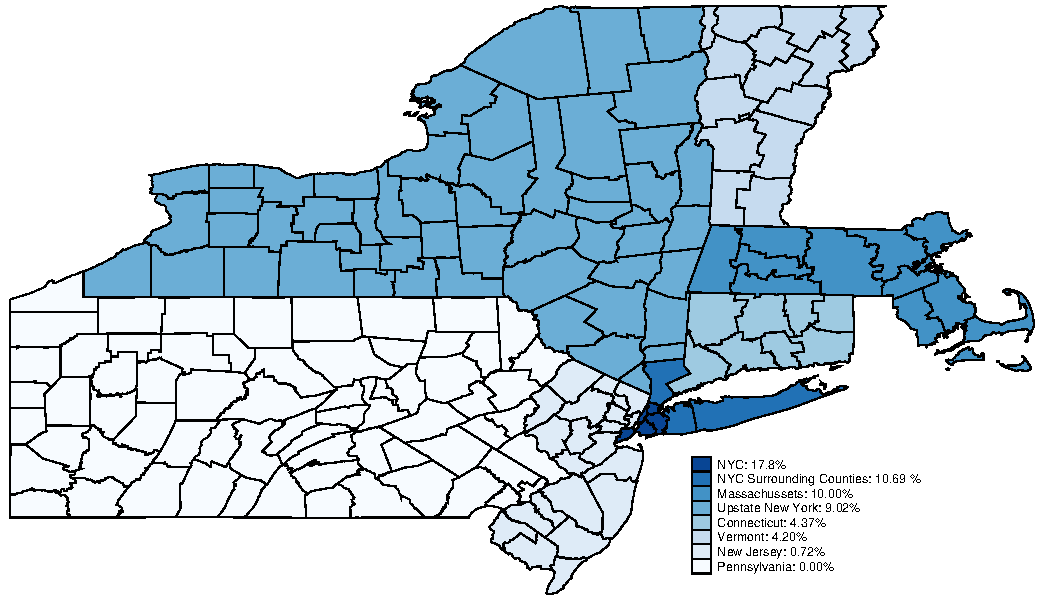
\includegraphics[scale=.65]{counties.pdf}

\end{frame}

\section{Data}

\begin{frame}{Data}
Yelp 
\begin{itemize}
\item Basic restaurant info, item and price info
\item Star rating 
\item Data collected: Apr `16, Jul `16, Oct `16, Jan `17, Feb `17
\end{itemize}

Grubhub
\begin{itemize}
\item Basic restaurant info, item and price info
\item Data collected: Dec `16, Jan `17, Feb `17
\end{itemize}

ReferenceUSA
\begin{itemize}
\item Business data
\item Sales, employees, restaurant type, franchise status
\end{itemize}

\end{frame}


\begin{frame}{Restaurant Definitions}

\begin{itemize}
\item Full service (FS): order after eating
\item Limited service (LS): order at the counter before eating
\item Chain: franchise status in ReferenceUSA dataset
\item Fast food = limited service + chain 
\end{itemize}
\end{frame}

\begin{frame}{Yelp Stars as Quality Measure}
\begin{itemize}
\item Main star rating: rounded average (to the .5 star) of consumer reviews
\item Actual start rating to the .1 is available online
\item Yelp has a proprietary algorithm to sort out fake reviews
\item One star increase in Yelp rating leads to a 5-9\% increase in revenue (Luca, 2016)
\item Yelp ratings of hospitals had significant correlations with industry standard measure of hospital quality as well as helath outcomes (Bardach et. al, 2013)
\end{itemize}
\end{frame}

\begin{frame}{Sample of Restaurants}

\centering
\small
\begin{tabular}{ccccccc } \\ \hline \hline
Source & N & \%LS  & \% Chain   & \% Small & Price \\ \hline \hline
&&& \\
RUSA & 89,114 & 19.94 & 14.06 & 75.72 & -\\
\\
Yelp (All) & 35,502 & 17.01 & 11.82 & 75.13& - \\
\\
Yelp (Prices) & 7,901 & 5.49  & 1.77 & 78.40 & 9.37 \\
\\ 
Grubhub  & 5,351 & 6.48 & 2.01 &  86.19 & 8.66 \\
\end{tabular}
\end{frame}

\begin{frame}{Sample Size by Min Wage Group}
\scriptsize
\centering
\begin{tabular}{c c c c c c } \\ \hline \hline
Area & \% Increase & Yelp Restaurants   & Grubhub Restaurants\\ \hline \hline
&&& \\
 NYC \& FF  & 14.29\% & 25   & 34 \\
 NY Upstate \& FF  & 10.26\% & 3&13 \\
NYC \& Lg & 22.22\% & 610 &  407\\
NYC \& Sm & 16.67 \% & 2,408 &  2,266\\
NYC MSA & 11.11\% & 425 &341\\
NY Upstate & 7.78\% & 378 &  207 \\
Connecticut & 5.21\% & 57  &  93 \\
New Jersey & 0.72\% & 1,479 & 792\\
Massachusetts & 10.00\% & 1,391 &  550\\
Pennsylvania & 0.00\% &  1,072 &  647\\
Vermont & 4.2\% & 50 & 2\\
\\ \hline
Total & & 7,901 &  5,351 \\
\end{tabular}
\end{frame}


\begin{frame}{Sample of Yelp Restaurants}

\centering
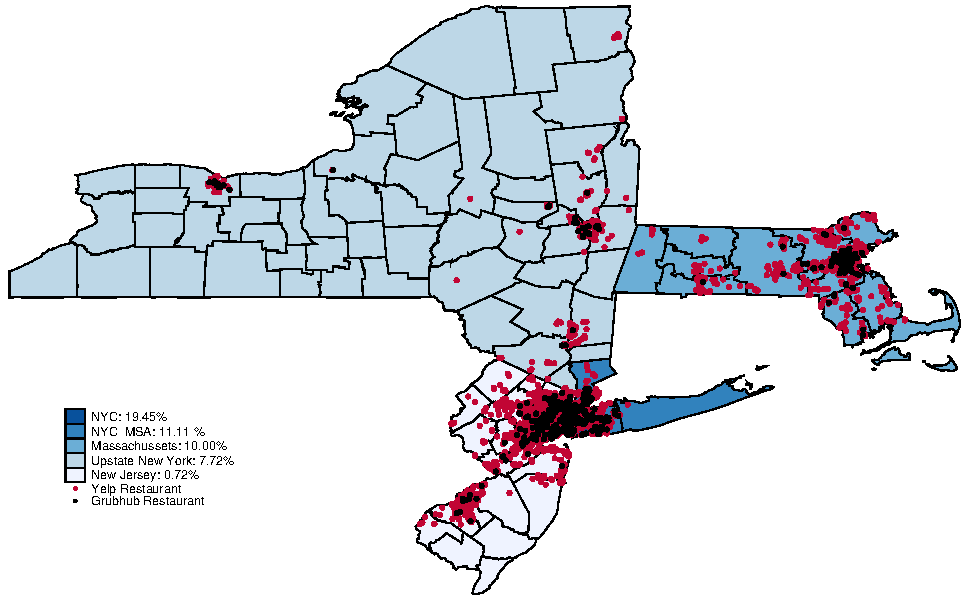
\includegraphics[scale=.65]{map_yelp.pdf}

\end{frame}

\section{Price Pass Through}

\begin{frame}{Expected Price Pass Through}
Assumptions:
\begin{itemize}
\item Factor markets competitive
\item Product markets competitive or monopolistically competitive
\item Firms have constant returns to scale production function
\end{itemize}

\bigskip

Price Pass Through:

\bigskip
\centering{($\% \Uparrow$ MW) $x$  ($\frac{MW Costs}{Labor Costs}$)  $x$  ($\frac{Labor Costs}{Total Costs}$) }

\bigskip
\centering{ (10\%) $x$ (17-33\%) $x$ (33\%) = 5.6-1.09\%}

\end{frame}

\begin{frame} {Model of Price Pass Through}

\begin{dmath}
\Delta \ln p_{ijkt} = \sum_{h=0}^{1}w_h \Delta \ln mw_{kt-h} +  \beta \Delta \ln p_{ijkt-1}  + \boldsymbol{X}_j \boldsymbol{\lambda} + \epsilon_k + \epsilon_t + \epsilon_{ijkt}
\end{dmath}

$i$ = item

$j$ = restaurant

$k$ = minimum wage group

$t$ = observation period

$\boldsymbol{X}_j$= vector of covariates: chain, LS, employees, sales, total items

\end{frame}




\begin{frame}{General Price Pass Through Results}
\centering
\scriptsize
{
\def\sym#1{\ifmmode^{#1}\else\(^{#1}\)\fi}
\begin{tabular}{l*{9}{c}}
\hline\hline
                    &\multicolumn{1}{c}{(1)}&\multicolumn{1}{c}{(2)}&\multicolumn{1}{c}{(3)}&\multicolumn{1}{c}{(4)}&\multicolumn{1}{c}{(5)}&\multicolumn{1}{c}{(6)}&\multicolumn{1}{c}{(7)}&\multicolumn{1}{c}{(8)}&\multicolumn{1}{c}{(9)}\\
                    &\multicolumn{1}{c}{ch\_lnp}&\multicolumn{1}{c}{ch\_lnp}&\multicolumn{1}{c}{ch\_lnp}&\multicolumn{1}{c}{ch\_lnp}&\multicolumn{1}{c}{ch\_lnp}&\multicolumn{1}{c}{ch\_lnp}&\multicolumn{1}{c}{ch\_lnp}&\multicolumn{1}{c}{ch\_lnp}&\multicolumn{1}{c}{ch\_lnp}\\
\hline
$ Oct - Jan $ &       0.0914\sym{**} &      0.0891\sym{*}  &       0.160\sym{*}  &       0.125         &     0.00553         &      0.0914\sym{**} &      0.0168\sym{***}&      0.0140\sym{***}&      0.0207\sym{***}\\
                    &    (0.0248)         &    (0.0477)         &    (0.0829)         &    (0.0844)         &     (0.107)         &    (0.0248)         &   (0.00110)         &   (0.00135)         &   (0.00169)         \\
[1em]
$Dec - Jan $&                     &      0.0585\sym{**} &   -0.000642         &     -0.0360         &      0.0489         &                     &      0.0225\sym{***}&      0.0219\sym{**} &      0.0285\sym{**} \\
                    &                     &    (0.0222)         &    (0.0438)         &    (0.0353)         &    (0.0512)         &                     &   (0.00230)         &   (0.00595)         &   (0.00671)         \\
[1em]
$Jan - Feb$&                     &      0.0661\sym{**} &   -0.000706         &     -0.0360         &      0.0315         &                     &      0.0153\sym{***}&      0.0255\sym{**} &      0.0321\sym{**} \\
                    &                     &    (0.0241)         &    (0.0370)         &    (0.0281)         &    (0.0316)         &                     &   (0.00196)         &   (0.00632)         &   (0.00783)         \\
      $Feb - March $ &                     &      0.0661\sym{**} &   -0.000706         &     -0.0360         &      0.0315         &                     &      0.0153\sym{***}&      0.0255\sym{**} &      0.0321\sym{**} \\
                    &                     &    (0.0241)         &    (0.0370)         &    (0.0281)         &    (0.0316)         &                     &   (0.00196)         &   (0.00632)         &   (0.00783)         \\
\hline
Observations        &      939186         &     1878373         &      623967         &      782051         &      782051         &     1408780         &     1465718         &     1465718         &     1465718         \\
\hline\hline
\multicolumn{10}{l}{\footnotesize Standard errors in parentheses}\\
\multicolumn{10}{l}{\footnotesize \sym{*} \(p<.10\), \sym{**} \(p<.05\), \sym{***} \(p<.001\)}\\
\end{tabular}
}

\end{frame}

\begin{frame}{Price Pass Through By Restaurant Characteristics \\ \large{Highest and Lowest Quartiles, Yelp}}
\centering
\tiny
{
\def\sym#1{\ifmmode^{#1}\else\(^{#1}\)\fi}
\begin{tabular}{l*{6}{c}}
\hline\hline
                    &\multicolumn{1}{c}{(1)}&\multicolumn{1}{c}{(2)}&\multicolumn{1}{c}{(3)}&\multicolumn{1}{c}{(4)}&\multicolumn{1}{c}{(5)}&\multicolumn{1}{c}{(6)}\\
                    &\multicolumn{1}{c}{Low Sales}&\multicolumn{1}{c}{High Sales}&\multicolumn{1}{c}{Low Emps}&\multicolumn{1}{c}{High Emps}&\multicolumn{1}{c}{Low Price}&\multicolumn{1}{c}{High Price}\\
\hline
$\Delta Ln(mw\_kt)$  &      0.0204\sym{**} &      0.0243\sym{***}&      0.0228\sym{***}&      0.0172\sym{***}&      0.0150\sym{**} &      0.0225\sym{***}\\
                    &   (0.00347)         &   (0.00189)         &   (0.00266)         &   (0.00190)         &   (0.00314)         &   (0.00288)         \\
[1em]
$\Delta Ln(mw\_kt-1)$&      0.0237\sym{**} &      0.0279\sym{*}  &      0.0276\sym{**} &      0.0167         &      0.0236\sym{**} &      0.0218\sym{**} \\
                    &   (0.00472)         &    (0.0127)         &   (0.00653)         &    (0.0158)         &   (0.00660)         &   (0.00915)         \\
[1em]
$\Delta Ln(mw\_{kt-2}) $&      0.0206\sym{**} &      0.0448\sym{**} &      0.0246\sym{**} &      0.0381\sym{**} &      0.0253\sym{**} &      0.0319\sym{**} \\
                    &   (0.00422)         &   (0.00895)         &   (0.00572)         &    (0.0100)         &   (0.00718)         &    (0.0120)         \\
\hline
Total Pass Through & 0.0647 & 0.0829 & 0.0750 & 0.0720 & 0.0639 & 0.0762 \\
Observations        &      437413         &      262235         &      541924         &      152959         &      362036         &      370341         \\
\hline\hline
\multicolumn{7}{l}{\footnotesize Standard errors in parentheses}\\
\multicolumn{7}{l}{\footnotesize \sym{*} \(p<.10\), \sym{**} \(p<.05\), \sym{***} \(p<.001\)}\\
\end{tabular}
}

\end{frame}


\begin{frame}{Price Change and Minimum Wage Increase \\\large{By Item Type, Grubhub}}
\centering
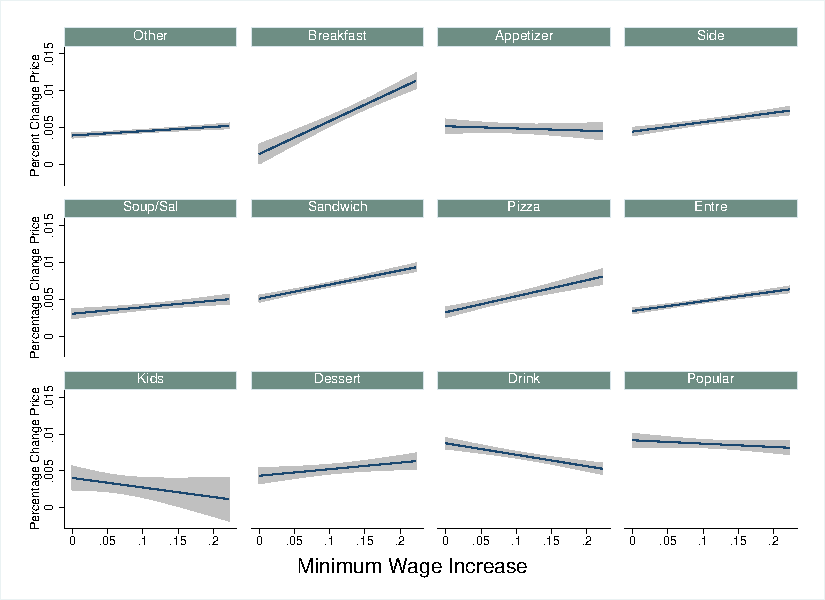
\includegraphics[width=3.5in]{grubhub_cats.pdf}
\end{frame}

\begin{frame}{Price Pass Through By Item Type \\ \small{Grubhub}}
\centering
\tiny
{
\def\sym#1{\ifmmode^{#1}\else\(^{#1}\)\fi}
\begin{tabular}{l*{7}{c}}
\hline\hline
                    &\multicolumn{1}{c}{(1)}&\multicolumn{1}{c}{(2)}&\multicolumn{1}{c}{(3)}&\multicolumn{1}{c}{(4)}&\multicolumn{1}{c}{(5)}&\multicolumn{1}{c}{(6)}&\multicolumn{1}{c}{(7)}\\
                    &\multicolumn{1}{c}{Popular}&\multicolumn{1}{c}{Side}&\multicolumn{1}{c}{Sandwich}&\multicolumn{1}{c}{Pizza}&\multicolumn{1}{c}{Entre}&\multicolumn{1}{c}{Desert}&\multicolumn{1}{c}{Drink}\\
\hline
$\Delta Ln(mw_{kt})$  &      0.0103         &     0.00797\sym{*}  &      0.0311\sym{**} &      0.0315\sym{**} &      0.0167\sym{***}&      0.0105         &     0.00847\sym{*}  \\
                    &   (0.00570)         &   (0.00289)         &   (0.00692)         &   (0.00605)         &   (0.00160)         &   (0.00745)         &   (0.00295)         \\
[1em]
$\Delta Ln(mw_{kt-1})$&      0.0577\sym{*}  &      0.0110\sym{*}  &      0.0387\sym{**} &      0.0436\sym{**} &      0.0247\sym{***}&      0.0273\sym{**} &      0.0383\sym{*}  \\
                    &    (0.0211)         &   (0.00385)         &   (0.00957)         &   (0.00894)         &   (0.00234)         &   (0.00751)         &    (0.0128)         \\
\hline
Observations        &       80588         &      148255         &      181206         &       61917         &      229315         &       29844         &       99171         \\
\hline\hline
%\multicolumn{8}{l}{\footnotesize Standard errors in parentheses}\\
%\multicolumn{8}{l}{\footnotesize \sym{*} \(p<0.05\), \sym{**} \(p<0.01\), \sym{***} \(p<0.001\)}\\
\end{tabular}
}

\end{frame}





\section{Quality}






\begin{frame}{Min Wage Impact on Yelp Star Ratings}

\begin{dmath}
\Delta \ln(exact\_stars_{jkt}) =\sum_{h=0}^{1}w_h \Delta \ln mw_{kt-h}  +   \sum_{h=0}^{1}\beta_h \Delta \ln p_{ijkt-h}  + \gamma stars\_july_{jkt} +\boldsymbol{X}_j  \boldsymbol{\lambda} + \epsilon_k + \epsilon_t + \epsilon_{ijkt}
\end{dmath}

$exact\_stars_{jkt}$: average star rating to the tenth

$stars\_july_{jkt}$: rounded average star rating


\end{frame}


\begin{frame}{Min Wage Impact on Yelp Star Ratings}
\centering
\scriptsize
<<<<<<< HEAD
\begin{center}
\begin{tabular}{lcccccc}
\hline  & (1) & (2) & (3) & (4) & (5) & (6)\\
 & All &  $ 2.5 $  &  $ 3.0 $  &  $ 3.5 $  &  $ 4.0 $  &  $ 4.5$ \\
\hline  $ Apr16-Jul16 $  & 0.035 & 1.138 & 0.625 & 0.068 & -1.047 & -0.627\\
 & (0.213) & (1.201) & (0.697) & (0.187) & (0.312) & (0.456)\\
 $ Jul16-Oct16 $  & -0.046 & -0.321 & -0.305 & 0.109 & 0.198 & -0.792\\
 & (0.071) & (0.292) & (0.400) & (0.211) & (0.296) & (0.413)\\
 $ Oct16-Jan17 $  & 0.049 & 0.255 & -1.341 & -0.268 & 0.500 & 0.470\\
 & (0.036) & (1.068) & (0.178) & (0.076) & (0.090) & (0.275)\\
 $ Jan17-Apr17 $  & -0.416 & -1.158 & -0.546 & -0.728 & -0.252 & -0.255\\
 & (0.167) & (0.609) & (0.670) & (0.197) & (0.080) & (0.175)\\
\hline \textit{Total \% Change Stars} & -0.368 & -0.903 & -1.887 & -0.996 & 0.248 & 0.215\\
  & (0.138) & (1.667) & (0.813) & (0.161) & (0.123) & (0.164)\\
\hline  $ N $  & 6392 & 625 & 1080 & 1801 & 1904 & 982\\
 $ NxT $  & 25568 & 2500 & 4320 & 7204 & 7616 & 3928\\
\hline\end{tabular}\\
\begin{tiny} \hfil\end{tiny}\\
\end{center}
=======
\begin{center}
\begin{tabular}{lcccccc}
\hline  & (1) & (2) & (3) & (4) & (5) & (6)\\
 & All &  $ 2.5 $  &  $ 3.0 $  &  $ 3.5 $  &  $ 4.0 $  &  $ 4.5$ \\
\hline  $ Apr16-Jul16 $  & 0.035 & 1.138 & 0.625 & 0.068 & -1.047 & -0.627\\
 & (0.213) & (1.201) & (0.697) & (0.187) & (0.312) & (0.456)\\
 $ Jul16-Oct16 $  & -0.046 & -0.321 & -0.305 & 0.109 & 0.198 & -0.792\\
 & (0.071) & (0.292) & (0.400) & (0.211) & (0.296) & (0.413)\\
 $ Oct16-Jan17 $  & 0.049 & 0.255 & -1.341 & -0.268 & 0.500 & 0.470\\
 & (0.036) & (1.068) & (0.178) & (0.076) & (0.090) & (0.275)\\
 $ Jan17-Apr17 $  & -0.416 & -1.158 & -0.546 & -0.728 & -0.252 & -0.255\\
 & (0.167) & (0.609) & (0.670) & (0.197) & (0.080) & (0.175)\\
\hline \textit{Total \% Change Stars} & -0.368 & -0.903 & -1.887 & -0.996 & 0.248 & 0.215\\
  & (0.138) & (1.667) & (0.813) & (0.161) & (0.123) & (0.164)\\
\hline  $ N $  & 6392 & 625 & 1080 & 1801 & 1904 & 982\\
 $ NxT $  & 25568 & 2500 & 4320 & 7204 & 7616 & 3928\\
\hline\end{tabular}\\
\begin{tiny} \hfil\end{tiny}\\
\end{center}
>>>>>>> 9bf80c4d3367c601bceb3268e37dc31cf9116a6c

\end{frame}


\begin{frame}{Change in Star Rating Distribution}
\centering
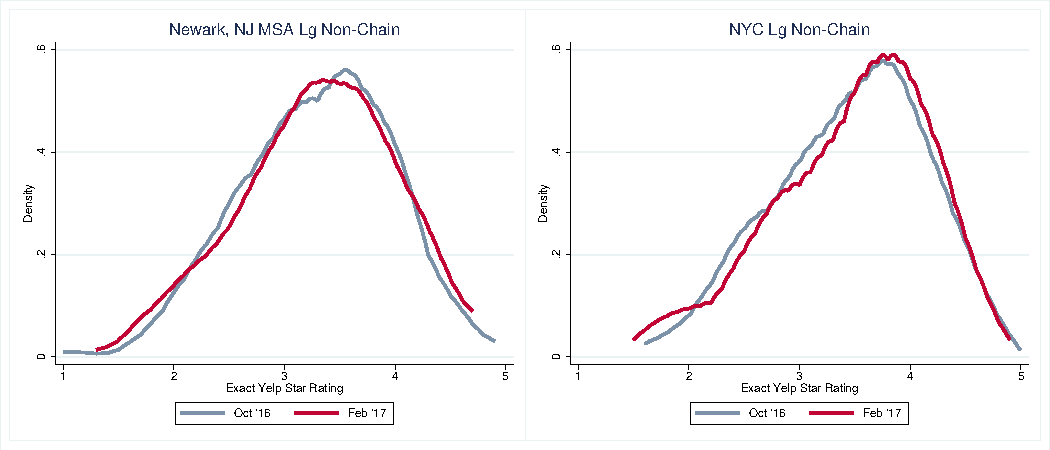
\includegraphics[width=4.5in]{star_densities.pdf}
\end{frame}

\begin{frame}{Other Non-Price Outcomes }
\small
\centering
{
\def\sym#1{\ifmmode^{#1}\else\(^{#1}\)\fi}
\begin{tabular}{l*{3}{c}}
\hline\hline
%                    &\multicolumn{1}{c}{(1)}&\multicolumn{1}{c}{(2)}&\multicolumn{1}{c}{(3)}\\
                    &\multicolumn{1}{c}{Hours}&\multicolumn{1}{c}{Days}&\multicolumn{1}{c}{Total Items}\\
\hline
$\Delta Ln(mw_{kt})$  &      -0.510         &     -0.0110         &      -3.426         \\
                    &     (0.706)         &    (0.0238)         &     (2.092)         \\
[1em]
$\Delta Ln(mw_{kt-1})$&     -0.0243         &     -0.0137         &      -7.295\sym{*}  \\
                    &     (0.897)         &    (0.0168)         &     (2.743)         \\
\hline
Observations        &       19373         &       19373         &       23217         \\
\hline\hline
%\multicolumn{4}{l}{\footnotesize Standard errors in parentheses}\\
%\multicolumn{4}{l}{\footnotesize \sym{*} \(p<0.05\), \sym{**} \(p<0.01\), \sym{***} \(p<0.001\)}\\
\end{tabular}
}

\end{frame}


\section{Border Effects}


\begin{frame}{Border Effects}

$$
\begin{aligned}
\Delta \ln (p_{ij,Feb-Oct})  = & \alpha_0 + \alpha_1  \mathbbm{1}(NY=1)  \\
& + \alpha_2 D_{j} + \alpha_3[D_j * \mathbbm{1}(NY=1)]  \\
& +\gamma X_{ij}  + \epsilon_{ij} 
\end{aligned}
$$

$D_j$: minutes to a competitor across the border

$\mathbbm{1}(NY=1)$: indicator function for state

\bigskip

\begin{centering}

NY: $
\Delta \ln (p_{ij,Feb-Oct})  = (\alpha_0 +\alpha_1) +  (\alpha_2 + \alpha_3) D_j +\gamma X_{ij}  + \epsilon_{ij}   
$

\bigskip

NJ:
$
\Delta \ln (p_{ij,Feb-Oct})  = (\alpha_0 ) +  (\alpha_2 ) D_j +\gamma X_{ij}  + \epsilon_{ij}   
$

\end{centering}
\end{frame}

\begin{frame}{Border Effects}

\centering
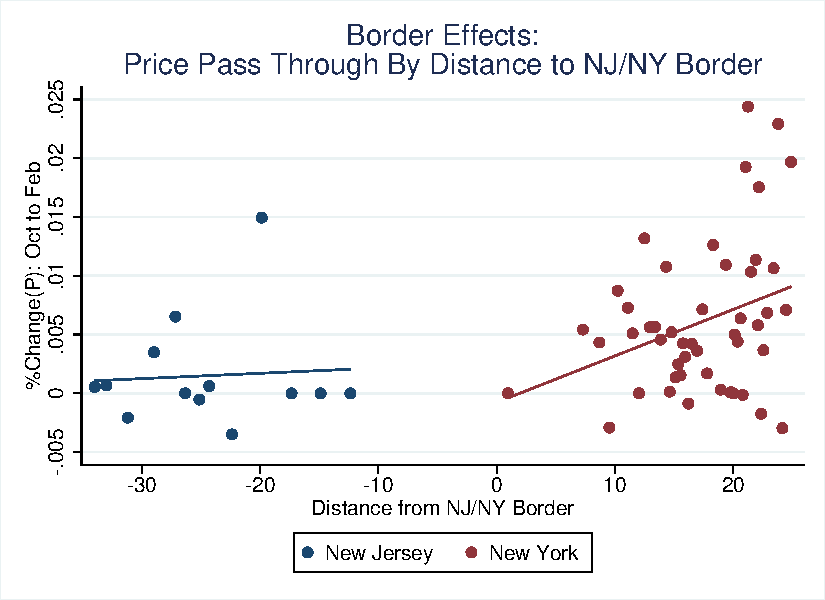
\includegraphics[width=4in]{total_pricechange_dist_nynj.pdf}
\end{frame}

\begin{frame}{Border Effects: Results}
\centering
\tiny
{
\def\sym#1{\ifmmode^{#1}\else\(^{#1}\)\fi}
\begin{tabular}{l*{4}{c}}
\hline\hline
                    &\multicolumn{1}{c}{(NJ)}&\multicolumn{1}{c}{(NJ)}&\multicolumn{1}{c}{(NJ)}&\multicolumn{1}{c}{(NY MSA)}\\
                    &\multicolumn{1}{c}{$\Delta Ln(P_{feb-oct})$}&\multicolumn{1}{c}{$\Delta Ln(P_{feb-oct})$}&\multicolumn{1}{c}{$\Delta Ln(P_{oct-jul})$}&\multicolumn{1}{c}{$\Delta Ln(P_{feb-oct})$}\\
\hline
Constant ($ \alpha_0 $)           &     0.00261         &     0.00268         &   -0.000689         &     0.00198         \\
                    &   (0.00145)         &   (0.00146)         &  (0.000873)         &   (0.00318)        \\
        [1em]
NYC ($ \alpha_1 $)     &    -0.00339\sym{*}  &    -0.00410\sym{*}  &     0.00218\sym{*}  &       -0.00589              \\
                    &   (0.00160)         &   (0.00161)         &  (0.000961)         &                     (0.00329)   \\
[1em]
Distance   ($\alpha_2$)            &   0.0000454         &   0.0000683         &  -0.0000366         &                      0.000245         \\
                    & (0.0000566)         & (0.0000568)         & (0.0000339)         &                     (0.000168)      \\
%[1em]
%ny=0 $\times$ dist\_nynj\_bord&           0         &           0         &           0         &                     \\
%                    &         (.)         &         (.)         &         (.)         &                     \\
[1em]
NYC $\times$ Distance ($\alpha_3$)    &    0.000350\sym{***}&    0.000322\sym{***}&   0.0000461         &     0.000293                 \\
                    & (0.0000678)         & (0.0000679)         & (0.0000405)         &                     (0.000177)   \\
%Chain               &                     &    -0.00553\sym{*}  &    -0.00222         &                     \\
%                    &                     &   (0.00243)         &   (0.00145)         &                     \\
%[1em]
%LS                  &                     &    -0.00383\sym{***}&    -0.00113\sym{*}  &                     \\
%                    &                     &  (0.000907)         &  (0.000542)         &                     \\
%[1em]
%Employees           &                     &  -0.0000586         &   0.0000367         &                     \\
%                    &                     & (0.0000472)         & (0.0000282)         &                     \\
%[1em]
%Sales               &                     &    2.48e-09\sym{***}&    1.82e-11         &                     \\
%                    &                     &  (4.42e-10)         &  (2.64e-10)         &                     \\
%[1em]
%nyc                 &                     &                     &                     &    -0.00589         \\
%                    &                     &                     &                     &   (0.00329)         \\
%[1em]
%dist\_nyny\_bord      &                     &                     &                     &    0.000245         \\
%                    &                     &                     &                     &  (0.000168)         \\
%[1em]
%nyc=0 $\times$ dist\_nyny\_bord&                     &                     &                     &           0         \\
%                    &                     &                     &                     &         (.)         \\
%[1em]
%nyc=1 $\times$ dist\_nyny\_bord&                     &                     &                     &    0.000293         \\
%                    &                     &                     &                     &  (0.000177)         \\
%[1em]
 \\
\hline
Observations        &       80402         &       80402         &       80402         &       23368         \\
\hline\hline
%	\multicolumn{5}{l}{\footnotesize Standard errors in parentheses}\\
%	\multicolumn{5}{l}{\footnotesize \sym{*} \(p<0.05\), \sym{**} \(p<0.01\), \sym{***} \(p<0.001\)}\\
\end{tabular}
}


\end{frame}

\begin{frame}{Border Effects: Interpretation}
For restaurants in NYC within 20 minutes of the NJ border...
\begin{itemize}
\item On average, a 1 minute increase in the distance from the NJ border \\ $\Rightarrow$ .0003 percentage point increase in $\%\Delta$ price 
\item On average, a 10 minute increase in the distance from the NJ border \\ $\Rightarrow$ .003 percentage point increase in $\%\Delta$ price 
\end{itemize}
Av$(\%\Delta(p))$ for all items in NYC from Oct to Feb = .0041

\end{frame}

\section{Conclusion}

\begin{frame}{Conclusion}
 How do restaurant prices change in response to increases in the minimum wage?
\begin{itemize}
\item Significant price pass through consistent with literature
\item Heterogeneity across restaurant characteristics
\item Heterogeneity across item type
\end{itemize}
 How is customer perceived quality of restaurants affected by a minimum wage increase?
\begin{itemize}
\item Good restaurants get better
\item Bad restaurants get worse
\end{itemize}
 Do border effects have an impact on price pass through?
\begin{itemize}
\item Yes, in areas with a minimum wage increase
\end{itemize}
\end{frame}





\end{spacing}
\end{document}











































